D'una funció $f(x)$, sabem que passa pel punt $(-1,-1)$ i que la gràfica de la seva funció derivada és la
següent:
\begin{center}
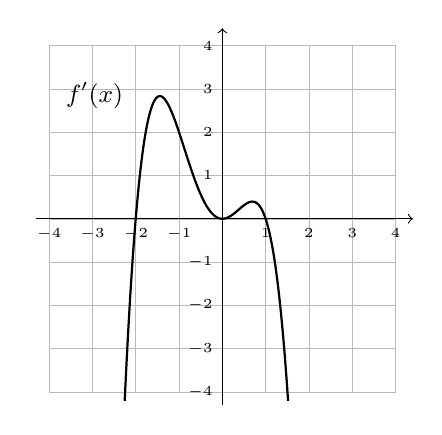
\begin{tikzpicture}[x=0.55cm,y=0.55cm]
  \draw[gray!55,very thin,step=1] (-4,-4) grid (4,4);
  \draw[->] (-4.3,0) -- (4.4,0);
  \draw[->] (0,-4.3) -- (0,4.4);
  \foreach \i in {-4,-3,-2,-1,1,2,3,4} \node[below,font=\tiny] at (\i,0) {$\i$};
  \foreach \j in {-4,-3,-2,-1,1,2,3,4} \node[left,font=\tiny] at (0,\j) {$\j$};
  \begin{scope}
    \clip (-4,-4.2) rectangle (4,4);
    \draw[\colorgrafica,thick,domain=-2.27:1.53,samples=160,smooth]
      plot (\x,{-(\x)*(\x)*((\x)+2)*((\x)-1)});
  \end{scope}
  \node[font=\small] at (-2.95,2.85) {$f'(x)$};
\end{tikzpicture}
\end{center}

\begin{apartats}

\apartat{1}
Calculeu l'equació de la recta tangent a la gràfica de la funció $f(x)$ en el punt $(-1,-1)$.

\begin{solucio}
Usarem l'expressió de la recta punt-pendent, $y-f(x_0)=m(x-x_0)$. Com que la recta buscada ha de passar pel
punt $x_0=-1$, $f(x_0)=-1$, hi ha de tenir pendent $f'(x_0)=f'(-1)=2$ (tal com es veu al gràfic), i
l'equació de la recta tangent a la funció $f(x)$ en el punt $x_0=-1$ serà
\[
y-(-1)=2\cdot\bigl(x-(-1)\bigr)\;\rightarrow\;y+1=2\cdot(x+1)\;\rightarrow\;y=2x+1 .
\]

\textit{Pauta oficial:} 0,5 per determinar el pendent de la recta tangent a partir del gràfic, i 0,5 per
l'equació de la recta.
\end{solucio}

\apartat{1}
Estudieu si $f(x)$ té punts crítics (punts on $f'(x)=0$) i, en cas que en tingui, determineu-ne les
abscisses i classifiqueu-los segons si són màxims, mínims o punts d'inflexió de $f(x)$.

\begin{solucio}
Els punts crítics de $f(x)$ són aquells que satisfan $f'(x)=0$. Del gràfic es veu clarament que són els
punts $x=-2$, $x=0$ i $x=1$: aquestes abscisses són possibles extrems relatius de la funció $f(x)$.\\
Com que $f'(x)$ és creixent en $x=-2$, la seva derivada en aquest punt serà positiva, $f''(-2)>0$, i això
vol dir que $x=-2$ és un mínim local de $f(x)$.\\
Anàlogament, com que $f'(x)$ és positiva immediatament abans de $x=1$ i negativa immediatament després, la
funció $f(x)$ és creixent abans de $x=1$ i decreixent després; per tant, $x=1$ és un màxim local de
$f(x)$.\\
El punt $x=0$ és diferent. Tant abans com després, $f'(x)$ és positiva, i per tant $f(x)$ és creixent en el
punt $x=0$. Però, a més, $f'(x)$ és decreixent abans de $x=0$, i per tant la seva derivada (és a dir,
$f''(x)$) és negativa, mentre que és creixent després de $x=0$, i per tant $f''(x)$ és positiva. Això vol
dir que la funció $f(x)$ és còncava abans de $x=0$ i convexa després. Per tant, el punt $x=0$ és un punt
d'inflexió de $f(x)$.

\textit{Pauta oficial:} 0,25 per la llista de punts crítics, 0,25 per deduir que $x=-2$ és un mínim, 0,25
per deduir que $x=1$ és un màxim i 0,25 per deduir que $x=0$ és un punt d'inflexió.
\end{solucio}

\apartat{0,5}
Sabent, a més, que $f(0)=-0{,}2$, calculeu l'àrea entre la gràfica de $f'(x)$ i l'eix de les abscisses, des
de $x=-1$ fins a $x=0$.

\begin{solucio}
Com que $f(x)$ és una primitiva de $f'(x)$, l'àrea que ens demanen és fàcil de calcular usant la regla de
Barrow (i usant les dades $f(0)=-0{,}2$ i $f(-1)=-1$):
\[
A=\int_{-1}^{0}f'(x)\,dx=\bigl[f(x)\bigr]_{-1}^{0}=f(0)-f(-1)=-0{,}2-(-1)=0{,}8\ \text{u}^2 .
\]

\textit{Pauta oficial:} 0,25 per reconèixer que $f(x)$ és una primitiva de $f'(x)$ i 0,25 pel càlcul de
l'àrea.

\textit{Nota del banc:} la corba dibuixada coincideix amb $f'(x)=-x^2(x+2)(x-1)$ (els zeros, $f'(-1)=2$ i
els extrems locals de $f'$). Amb aquesta expressió, l'àrea exacta seria $\int_{-1}^{0}f'(x)\,dx=\frac{43}{60}
\approx0{,}72\ \text{u}^2$, i no 0,8: la dada $f(0)=-0{,}2$ de l'enunciat no és del tot coherent amb el dibuix.
L'exercici, però, demana fer servir aquesta dada, i la resposta esperada és 0,8.
\end{solucio}

\end{apartats}
